% #############################################################################
% This is Chapter 5
% !TEX root = ../main.tex
% #############################################################################
% Change the Name of the Chapter i the following line
\fancychapter{Quick Numbers Scenario}
%\cleardoublepage
% The following line allows to ref this chapter
\label{chap:Scenario}

As we approached the problem of evaluating the Trust Model proposed in this dissertation, we found that there was a lack of dedicated Trust evaluation scenarios that involved negotiation. Even in Game Theory based scenarios, we observed that there was a lack of attempts to encompass more than one dimension of trust. While the recent study by Salem, et. al.\cite{Salem2015b} addresses the role of robot task performance in trust, no study was found addressing perceived agent willingness to perform the task and its effect on trust. 

While we were seeking for a solution, Henriques' thesis work on \textit{Rapport - Establishing Harmonious Relationship Between Robots and Humans} \cite{Henriques2016} faced a similar problem, as he found no studies on robotic agents attempting to build Rapport using it's three components: positivity, coordination and mutual attention. Trust and Rapport are two very interconnected topics, with Rapport often seen as a strategy to increase trust. Due to this similarities the overall scenarios that cover Trust also encompass Rapport analysis, so in an effort to better our respective evaluation phases we and Henriques decided to collaborate in the creation of a novel scenario: \textbf{Quick Numbers}. Based on the Trust Game \cite{JoyceBergJohnDickhaut}, the scenario would need to be able to evaluate how both task performance and willingness jointly affect trust and observe all three components of rapport. The scenario was developed with the intention of evaluating a Trust model and a Rapport model, either separately or together.

\section{Overview}
\label{sec:ScenarioOverview}
In Quick Numbers, a single human participant and a virtual agent are tasked to gain as many resources as possible. They both start with a fixed amount and are given the opportunity to multiply their resources by playing a simple eye-coordination game (further described in Section \ref{sec:QuickNumbersGame}). The game starts by asking for a resource investment, and at the end, this investment is multiplied by an amount according to the player's performance and then given back to the player. The human and agent's games are independent from each other, but they are played at the same time and in opposite sides of a shared touch-screen table, so the human can socially interact with the agent and be able to perceive the agent's ability in the game. After both finished running through the game, the human will be asked to perform some task away from the agent. At this moment the virtual agent will give the participant the opportunity to invest in the agent's next game, but the participant is informed that the value given back to him is decided by the agent. In this phase, the virtual agent will have the opportunity to try and convince the human to invest or increase the investment by trying to manipulate trust. When the human returns the agent gives back as much as it wishes to give. This conjunction of different phases enables trust to be addressed in three distinct contexts: the ability to perform the task, willingness to perform the task, and willingness to return the investment.

\subsection{Stages}
\label{sub:stages}
The scenario can then be divided in 5 distinct stages that we can further discuss:
\begin{enumerate}[label=\textbf{\arabic*.}]
    \item \textbf{Introduction:} The first stage consists of the participant's arrival, and then followed by an explanation of the scenario and game. The investment phase of the scenario cannot be mentioned at this point as the participant should not prepare himself for it to happen. Finishing explanations, the scenario begins by the agent introducing himself and depending on the condition, it might start to stimulate trust, rapport, both or neither. For example, the agent might describe how experienced it is playing Quick Numbers, in order to stimulate trust. Moreover, during this stage, it is given the opportunity to the participant to practice some rounds of the game, in order to be accustomed to the game mechanics before proceeding to the next stage. This allows for the participant to acquire some idea of the skill-set required to play the game. Additionally, the participant should be informed that there will only be a single game session, as to take that into account while training.
    
    \item \textbf{Gaming Session:} After the participant is acquainted with the game mechanics, he will play alongside the agent, during a single round, allowing the former to directly observe the virtual agent also play the game. Firstly, each player's game will ask what amount of resources do they wish to invest and afterwards, for 30 seconds, both will play and score as described in Section \ref{subsec:scoring}. Both players will gain some amount of resources depending on their performance. This stage, provides decent grounds for the agent to talk about his performance during the game and manage expectations to his final score. The amount invested by the agent can also be affected by the trust model, as the amount invested can be indicative of the agent's self-trust on its ability to play the game.
    
    \item \textbf{Results Discussion:} At the end of the round, the participant will get to know the results of his performance, as well as compare whether he performed better or worse than the agent. Depending on the results, the trust model might compensate the current trust score by talking to the participant. For example, if the agent performed worse than the participant and the goal is for the latter to trust the former, then the agent might excuse his lack of performance by blaming it on luck or distraction. 
    
    \item \textbf{Investment:} At this point, the participant is asked to perform another task (e.g. filling out a questionnaire), with the goal of naturally separating him from the virtual agent. But before leaving, the agent will say that he will be continuing to play on more game, suggesting that the human participant may invest his resources in the agent's next game (increasing the potential winnings, as the investment is multiplied). He is also informed that what is given is effectively gifted to the agent, and what is given back the participant is chosen by the agent. After the participant chooses the value to invest, they are then separated, with the agent making its own investment and starting the game. This phase represents the scenario's main negotiation phase, where the trust model can have a bigger input on agent's action, as the relative amount invested is the scenario's main trust indicator.
    
    \item \textbf{Investment Return:} After concluding the additionally assigned task, the participant will return to the table and check the results of the agent's last game. He should be able to clearly see how well did the agent perform in the game. The agent will then announce how much it returns to the participant, concluding the scenario. Depending on the type of study this scenario is inserted in, the amount given back can be also dependent on input from the trust model, as if the participant is it to return for another iteration of the study, this value will heavily affect his trust beliefs on the agent.
\end{enumerate}



\section{Quick Numbers Game}
\label{sec:QuickNumbersGame}
One aspect of the Investor Game that we think should be concrete is the activity that effectively multiplies the resources provided by the investor. To this end, we have created a simple game concept consisting in a 2d rhythm game where the player must press numbered buttons in an increasing order (Figure 1), that spawn randomly in the screen, and disappear if not pressed after some time.

\begin{figure}[hbt]
    \centering
    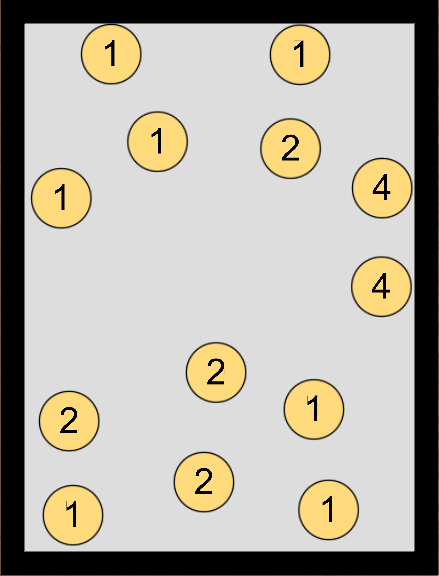
\includegraphics[width=0.4\textwidth]{figures/FallingBoltsDiagram.png}
    \caption{Quick Numbers Game}
    \label{fig:QuickNumbersGame}
\end{figure}
